\documentclass[tikz,border=10pt]{standalone}
\usepackage{amsmath}
\usetikzlibrary{arrows.meta, positioning, calc, decorations.pathreplacing}

\definecolor{c1}{HTML}{000000}
\definecolor{c2}{HTML}{233D4D}
\definecolor{c3}{HTML}{FE7F2D}
\definecolor{c4}{HTML}{EAECF0}
\definecolor{axiscolor}{HTML}{333333}
\definecolor{labelcolor}{HTML}{5F6B75}

\begin{document}
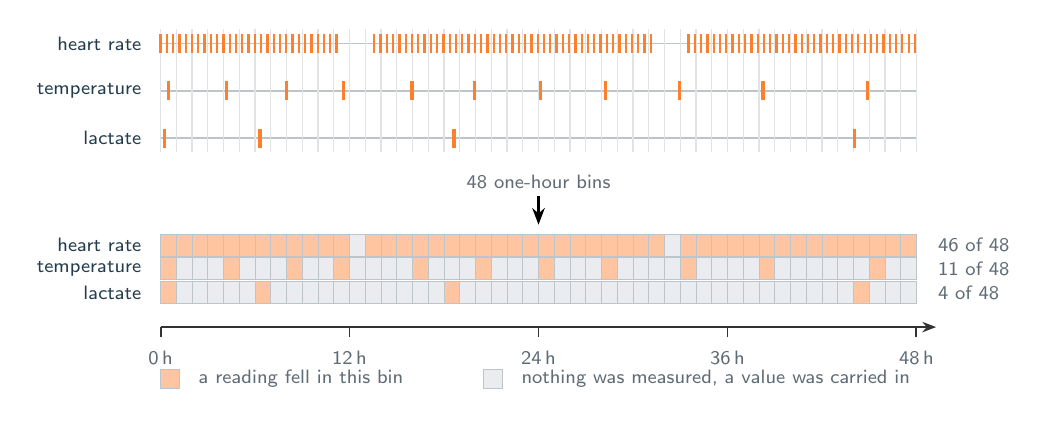
\begin{tikzpicture}[
    every node/.style={font=\sffamily},
    lab/.style={font=\sffamily\scriptsize, text=labelcolor},
    tag/.style={font=\sffamily\scriptsize, text=c2},
    hot/.style={font=\sffamily\scriptsize, text=c3!85!black},
]

\def\X#1{1.20 + #1*0.003333}
\def\B#1{1.20 + #1*0.200}

% ---------------------------------------------------------------- the chart
\foreach \y/\name in {6.00/heart rate, 5.40/temperature, 4.80/lactate}{
    \node[tag, anchor=east] at (1.08, \y) {\name};
    \draw[c2!30, line width=0.6pt] (1.20, \y) -- (10.80, \y);
}
\foreach \b in {0,...,48}{
    \draw[c2!14, line width=0.4pt] ({\B{\b}}, 4.62) -- ({\B{\b}}, 6.18);
}
\foreach \m in {0,24,...,2880}{
    \pgfmathparse{((\m>690)&&(\m<810)) || ((\m>1890)&&(\m<2010)) ? 0 : 1}
    \ifnum\pgfmathresult=1
        \draw[c3, line width=0.8pt] ({\X{\m}}, 5.88) -- ({\X{\m}}, 6.12);
    \fi
}
\foreach \m in {30, 250, 480, 700, 960, 1200, 1450, 1700, 1980, 2300, 2700}{
    \draw[c3, line width=1.1pt] ({\X{\m}}, 5.28) -- ({\X{\m}}, 5.52);
}
\foreach \m in {15, 380, 1120, 2650}{
    \draw[c3, line width=1.3pt] ({\X{\m}}, 4.68) -- ({\X{\m}}, 4.92);
}
\node[lab, anchor=north] at (6.00, 4.46) {48 one-hour bins};

\draw[{Stealth[length=6pt]}-, line width=1.0pt, c1] (6.00, 3.70) -- (6.00, 4.06);

% ---------------------------------------------------------------- the matrix
\foreach \y/\name in {3.30/heart rate, 3.00/temperature, 2.70/lactate}{
    \node[tag, anchor=east] at (1.08, {\y+0.14}) {\name};
    \foreach \b in {0,...,47}{
        \filldraw[draw=c2!30, fill=c4, line width=0.3pt]
            ({\B{\b}}, \y) rectangle ({\B{\b}+0.20}, {\y+0.28});
    }
}
% bins that actually contain a reading
\foreach \b in {0,1,...,11}{
    \filldraw[draw=c2!30, fill=c3!45, line width=0.3pt]
        ({\B{\b}}, 3.30) rectangle ({\B{\b}+0.20}, 3.58);
}
\foreach \b in {13,14,...,31}{
    \filldraw[draw=c2!30, fill=c3!45, line width=0.3pt]
        ({\B{\b}}, 3.30) rectangle ({\B{\b}+0.20}, 3.58);
}
\foreach \b in {33,34,...,47}{
    \filldraw[draw=c2!30, fill=c3!45, line width=0.3pt]
        ({\B{\b}}, 3.30) rectangle ({\B{\b}+0.20}, 3.58);
}
\foreach \b in {0,4,8,11,16,20,24,28,33,38,45}{
    \filldraw[draw=c2!30, fill=c3!45, line width=0.3pt]
        ({\B{\b}}, 3.00) rectangle ({\B{\b}+0.20}, 3.28);
}
\foreach \b in {0,6,18,44}{
    \filldraw[draw=c2!30, fill=c3!45, line width=0.3pt]
        ({\B{\b}}, 2.70) rectangle ({\B{\b}+0.20}, 2.98);
}

\node[lab, anchor=west] at (10.95, 3.44) {46 of 48};
\node[lab, anchor=west] at (10.95, 3.14) {11 of 48};
\node[lab, anchor=west] at (10.95, 2.84) {4 of 48};

% ---------------------------------------------------------------- axis
\draw[axiscolor, line width=0.8pt, -{Stealth[length=5pt]}]
    (1.20, 2.40) -- (11.05, 2.40);
\foreach \h in {0, 12, 24, 36, 48}{
    \draw[axiscolor, line width=0.7pt] ({\B{\h}}, 2.40) -- ({\B{\h}}, 2.28);
    \node[lab, anchor=north] at ({\B{\h}}, 2.22) {\h\,h};
}

% ---------------------------------------------------------------- legend
\filldraw[draw=c2!30, fill=c3!45, line width=0.3pt] (1.20, 1.62) rectangle (1.44, 1.86);
\node[lab, anchor=west] at (1.56, 1.74) {a reading fell in this bin};
\filldraw[draw=c2!30, fill=c4, line width=0.3pt] (5.30, 1.62) rectangle (5.54, 1.86);
\node[lab, anchor=west] at (5.66, 1.74) {nothing was measured, a value was carried in};

\end{tikzpicture}
\end{document}
